\documentclass{../../oss-apphys-exam}
\newcounter{last}

\begin{document}
%\genheader

\gentitle{12}{PLANETARY MOTION}

%\genmultidirections
%\gengravity

\raggedcolumns
\begin{multicols*}{2}
  \begin{questions}
    \question The Earth is at an average distance of \SI1{AU} from the Sun and
    has an orbital period of \SI1{year}. Jupiter orbits the Sun at
    approximately \SI5{AU}. About how long is the orbital period of Jupiter?
    \begin{choices}
      \choice\SI1{year}
      \choice\SI2{years}
      \choice\SI5{years}
      \choice\SI{11}{years}
      \choice\SI{125}{years}
    \end{choices}
    
    \question A satellite orbits the Earth at a distance of
    \SI{200}{\kilo\metre} in a circular path. If the mass of the Earth is
    \SI{6.e24}{\kilo\gram} and the Earth's radius is \SI{6.4e6}\metre, what is
    the satellite's speed?
    \begin{choices}
      \choice\SI{1.e3}{\metre\per\second}
      \choice\SI{3.5e3}{\metre\per\second}
      \choice\SI{7.8e3}{\metre\per\second}
      \choice\SI{5e6}{\metre\per\second}
      \choice\SI{6.1e7}{\metre\per\second}
    \end{choices}
    
    \question A satellite orbits the Earth in an elliptical orbit, with point A
    being close to the Earth and point B farther away. As the satellite moves
    from point A to point B, which of the following is true of the angular
    momentum and kinetic energy of the satellite?
    \begin{center}
      \vspace{-.1in}
      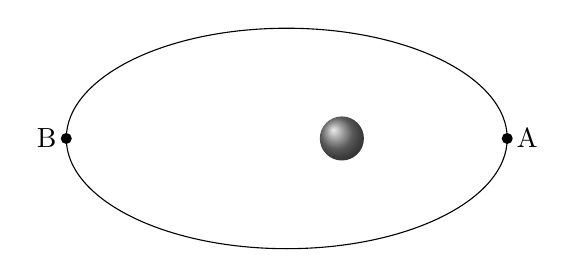
\begin{tikzpicture}[scale=1.4]
        \draw ellipse (2 and 1);
        \fill ( 2,0) circle(.05) node[right]{A};
        \fill (-2,0) circle(.05) node[left]{B};
        \shade[ball color=gray](.5,0) circle(.2);
      \end{tikzpicture}
    \end{center}
  
    \begin{tabular}{lll}
      & \underline{Angular momentum} & \underline{Kinetic energy}\\
      (A) & Increases & Remains constant \\
      (B) & Remains constant & Increases \\
      (C) & Decreases & Remains constant \\
      (D) & Remains constant & Decreases \\
      (E) & Remains constant & Remains constant
    \end{tabular}
    \columnbreak
    
    \question A satellite is in a stable circular orbit around the Earth at a
    radius $R$ and speed $\varv$. At what radius would the satellite travel in
    a stable orbit with a speed $2\varv$?
    \begin{choices}
      \choice $\dfrac R4$
      \choice $\dfrac R2$
      \choice $R$
      \choice $2R$
      \choice $4R$
    \end{choices}
    
    \question Two planets, X and Y, orbit a star. Planet X orbits at a radius
    $R$, and Planet Y orbits at a radius $3R$. Which of the following best
    represents the relationship between the acceleration $a_X$ of Planet X and
    the acceleration $a_Y$ of Planet Y?
    \begin{center}
      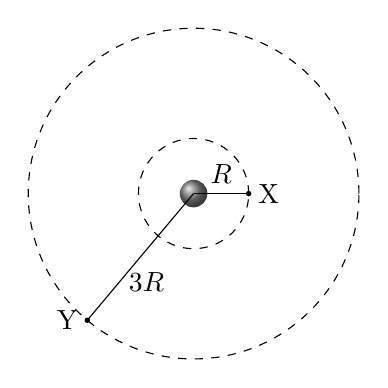
\begin{tikzpicture}[scale=.7]
        \shade[ball color=gray] circle(.25);
        \draw[dashed] circle(1);
        \draw[dashed] circle(3);
        \draw(0,0)--(1,0) node[right]{X} node[midway,above]{$R$};
        \fill(1,0) circle(.05);
        \begin{scope}[rotate=230]
          \draw(0,0)--(3,0) node[left]{Y} node[pos=.7,right]{$3R$};
          \fill(3,0) circle(.05);
        \end{scope}
      \end{tikzpicture}
    \end{center}
    \begin{choices}
      \choice $a_X = 9a_Y$
      \choice $9a_X = a_Y$
      \choice $a_X = 3a_Y$
      \choice $3a_X = a_Y$
      \choice $a_X = a_Y$
    \end{choices}
    
    \question A planet orbits at a radius $R$ around a star of mass $M$. The
    period of orbit of the planet is
    \begin{choices}
      \choice $\sqrt{\dfrac{4\pi^2R^2}{GM}}$
      \choice $\dfrac{4\pi^2R^3}{GM}$
      \choice $\sqrt{\dfrac{4\pi^2R^3}{GM}}$
      \choice $\sqrt{\dfrac{4\pi^2R}{GM}}$
      \choice $\dfrac{GM}{4\pi^2R}$
    \end{choices}
    \columnbreak
    
    \question A moon orbits a large planet in an elliptical orbit, with its
    closest approach at a distance $a$, and its farthest distance $b$. The
    speed of the moon at point $b$ is $\varv$. The speed at point $a$ is
    \begin{choices}
      \choice $\dfrac{a\varv}b$
      \choice $\dfrac{b\varv}a$
      \choice $\dfrac{(a+b)\varv}b$
      \choice $\dfrac{(b-a)\varv}b$
      \choice $\dfrac{2b\varv}a$
    \end{choices}

    \question A satellite orbits the Earth in an elliptical orbit. Which of the
    following statements is true?
    \begin{choices}
      \choice The angular velocity of the satellite increases as it travels
      farther from the Earth.
      \choice The acceleration of the satellite increases as it travels closer
      to the Earth.
      \choice The angular momentum of the satellite increases as it travels
      closer to the Earth.
      \choice The potential energy of the satellite is equal to its kinetic
      energy at all points in the orbit.
      \choice The speed of the satellite must remain constant for it to remain
      in orbit around the Earth.
    \end{choices}
    \vspace{.7in}
    
    \question A satellite of mass $m$ travels in an elliptical orbit around a
    planet of mass $M$. The satellite has a speed $\varv$ when it is closest to
    the planet at a distance $r$. Work is done by the engines of the satellite
    to change its orbit to a circular orbit when it is at this distance $r$.
    Which of the following statements is true of the transition from an
    elliptical orbit to a circular orbit?
    \begin{choices}
      \choice The work done by the satellite engines to change the orbit is
      equal to the change in kinetic energy of the satellite.
      \choice The work done by the satellite engines to change the orbit is
      equal to the change in potential energy of the satellite.
      \choice The work done by the satellite engines to change the orbit is
      equal to the change in angular momentum of the satellite.
      \choice The work done by the satellite engines to change the orbit is
      equal to the change in speed of the satellite.
      \choice The work done by the satellite engines to change the orbit is
      equal to the change in orbital radius of the satellite.
    \end{choices}
    \columnbreak
    
    \question A satellite of mass $m$ orbits the Earth with a potential energy
    $U$ and a kinetic energy $K$. Which of the following statements would have
    to be true for the satellite to escape the Earth's gravity completely?
    \begin{choices}
      \choice The kinetic energy of the satellite would have to be equal to the
      potential energy between the Earth and the satellite.
      \choice The potential energy between the Earth and the satellite would
      have to be greater than the kinetic energy of the satellite.
      \choice The total energy of the satellite would have to be greater than
      the kinetic energy of the satellite.
      \choice The kinetic energy of the satellite would have to be greater than
      the potential energy of the satellite.
      \choice The total energy of the satellite would have to be equal to the
      potential energy of the satellite.
    \end{choices}
  \end{questions}
  \setcounter{last}{\value{question}}
\end{multicols*}
\newpage

%\genfreetitle{12}{UNIVERSAL GRAVITATION}{2}
%\genfreedirections

\begin{questions}
  \setcounter{question}{\value{last}}
  
  % TAKEN FROM THE 2007 AP PHYSICS C MECHANICS EXAM FREE-RESPONSE QUESTION 2
  \question In March 1999 the Mars Global Surveyor (GS) entered its final orbit
  about Mars, sending data back to Earth. Assume a circular orbit with a period
  of $\SI{1.18e2}\minute=\SI{7.08e3}\second$ and orbital speed of
  \SI{3.40e3}{\metre\per\second}. The mass of the GS is \SI{930}{\kilo\gram}
  and the radius of Mars is \SI{3.43e6}\metre.
  \begin{parts}
    \part Calculate the radius of the GS orbit.
    \vspace{\stretch1}
    
    \part Calculate the mass of Mars.
    \vspace{\stretch1}
    
    \part Calculate the total mechanical energy of the GS in this orbit.
    \vspace{\stretch1}
    
    \part If the GS was to be placed in a lower circular orbit (closer to the
    surface of Mars), would the new orbital period of the GS be greater than or
    less than the given period?
    
    \vspace{.15in}
    \underline{\hspace{.3in}} Greater than\hspace{1in}
    \underline{\hspace{.3in}} Less than

    \vspace{.15in} Justify your answer.
    \vspace{\stretch1}
    
    \part In fact, the orbit the GS entered was slightly elliptical with its
    closest approach to Mars at \SI{3.71e5}{\metre} above the surface and its
    furthest distance at \SI{4.36e5}{\metre} above the surface. If the speed of
    the GS at closest approach is \SI{3.40e3}{\metre\per\second}, calculate the
    speed at the furthest point of the orbit.
    \vspace{\stretch1}
  \end{parts}
  \newpage
  
  % TAKEN FROM THE 2005 AP PHYSICS C MECHANICS EXAM FREE-RESPONSE QUESTION 2
  \question A student is given the set of orbital data for some of the moons of
  Saturn shown below and is asked to use the data to determine the mass $M_S$
  of Saturn. Assume the orbits of these moons are circular.
  \begin{center}
    \def\arraystretch{1.7}
    \begin{tabular}{|c|c|p{1in}|p{1in}|}
      \hline
      Orbital Period, $T$ (\si\second) & Orbital Radius, $R$ (\si\metre) & & \\
      \hline
      \num{8.14e4} & \num{1.85e8} & & \\ \hline
      \num{1.18e5} & \num{2.38e8} & & \\ \hline
      \num{1.63e5} & \num{2.95e8} & & \\ \hline
      \num{2.37e5} & \num{3.77e8} & & \\ \hline
    \end{tabular}
  \end{center}
  \def\arraystretch{1}
  \begin{parts}
    \part Write an algebraic expression for the gravitational force between
    Saturn and one of its moons.
    \label{algebraic}
    \vspace{\stretch1}
    
    \part Use your expression from part (\ref{algebraic}) and the assumption of
    circular orbits to derive an equation for the orbital period $T$ of a moon
    as a function of its orbital radius $R$.
    \vspace{\stretch1}
    
    \part Which quantities should be graphed to yield a straight line whose
    slope could be used to determine Saturn's mass?
    \vspace{\stretch1}
    
    \part Complete the data table by calculating the two quantities to be
    graphed. Label the top of each column, including units.
    \vspace{\stretch1}
    \newpage
    
    \part Plot the graph on the axes below. Label the axes with the variables
    used and appropriate numbers to indicate the scale.
    \begin{center}
      \begin{tikzpicture}[xscale=.48,yscale=.35]
        \draw[axes] (0,0)--(31,0);
        \draw[axes] (0,0)--(0,31);
        \draw[gray,help lines] grid(30,30);
        \draw[thick,step=5] grid(30,30);
      \end{tikzpicture}
    \end{center}
    \vspace{.4in}
    \part Using the graph, calculate a value for the mass of Saturn.
  \end{parts}
%  \newpage
%  
%  \question\textbf{THIS IS A CHALLENGE PROBLEM THAT IS MORE DIFFICULT THAN AP
%    EXAMS:} Spacecraft that study the Sun are often placed at the ``L1 Lagrange
%  Point'', located sunward of Earth on the Sun--Earth line. L1 is the point
%  where Earth's and Sun's gravity together produce an orbital period of one
%  year, so that a spacecraft at L1 stays fixed relative to Earth as both planet
%  and spacecraft orbit the Sun. This placement ensures an uninterrupted view of
%  the sun, without being periodically eclipsed by Earth as would occur in Earth
%  orbit. Find L1's location relative to Earth. (Hint: This problem calls for
%  numerical methods for solving high-order polynomial equation.)
\end{questions}
\end{document}
